\documentclass[landscape]{article}
\usepackage{graphicx,amssymb,color}
\pagestyle{empty}
\oddsidemargin  -0.5 in
\evensidemargin -0.5 in
\headheight     0 in
\topmargin      -1 in
\textheight     7.7 in
\textwidth      10 in
\newenvironment{slide}[1][ ]{\mbox{\boldmath \bf #1 } \vfill}{\vfill \mbox{ } \pagebreak}
\begin{document}
\huge \sf
\renewcommand{\labelitemi}{{\LARGE $\stackrel{\bullet}{\mbox{ }}$}}
\setlength{\parindent}{0 cm}

\begin{slide}

\begin{center}
  \Huge Final Update on \boldmath $\Gamma_{ee}$

  \vspace{1 cm}
  Jim Pivarski
\end{center}

\end{slide}

\begin{slide}[Reminder of $\Gamma_{ee}$]

$\Gamma_{ee} = \displaystyle \frac{{M_\Upsilon}^2}{6\pi^2} \int \sigma(e^+e^- \to
\Upsilon) \, dE$, integral from cross-section versus energy fits

\vfill
\begin{center}
  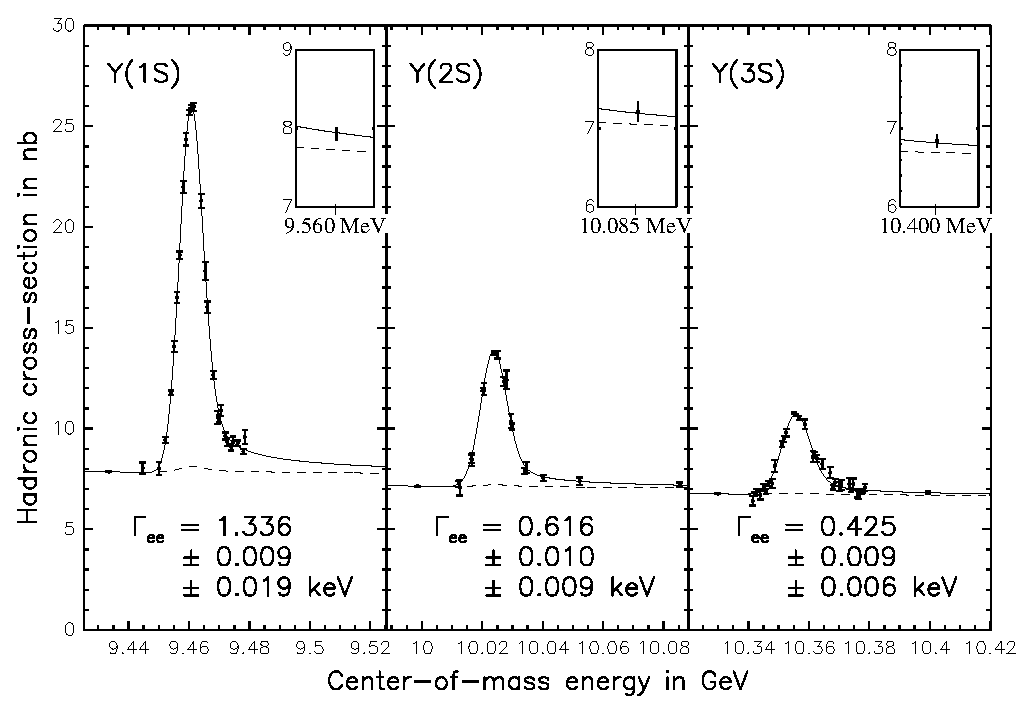
\includegraphics[width=0.8\linewidth]{../panic05/xfiged_three_resonances_inset_squat2}
\end{center}

\vfill
This result went to EPS, Lattice05, and will go to PANIC05

\vspace{-1 cm}

\end{slide}

\begin{slide}

What went into this measurement?

\vspace{1 cm}
\begin{itemize}\setlength{\itemsep}{1 cm}

  \item Scan procedures designed to minimize uncertainty from beam energy: $\lesssim$ 0.2\%

  \item Background subtraction with 0.25\% uncertainty

  \item $\Upsilon$ efficiency with 0.7\% uncertainty

  \item Luminosity calibration with 1.3\% uncertainty

\end{itemize}

\vspace{2 cm}
Luminosity calibration and most of efficiency systematics cancel in ratios of $\Gamma_{ee}(nS)/\Gamma_{ee}(mS)$

Ratios have 2--3\% statistical uncertainties

\vspace{1 cm}
The ratios are also easier for Lattice QCD to predict

\end{slide}

\begin{slide}[Reducing Statistical Uncertainties]

Preliminary results used $e^+e^- \to \gamma\gamma$ for point-by-point (relative) luminosity

which dominates statistical uncertainty

\vfill
Improve measurement with $e^+e^- \to e^+e^-$

\vfill
\begin{center}
  \renewcommand{\arraystretch}{2}
  \begin{tabular}{c c c c}
    & \hspace{0.25 cm} $\Gamma_{ee}(2S)/\Gamma_{ee}(1S)$ \hspace{0.25 cm} & \hspace{0.25 cm} $\Gamma_{ee}(3S)/\Gamma_{ee}(1S)$ \hspace{0.25 cm} & \hspace{0.25 cm} $\Gamma_{ee}(3S)/\Gamma_{ee}(2S)$ \hspace{0.25 cm} \\\hline
    $e^+e^- \to \gamma\gamma$ & 1.7\% & 2.3\% & 2.7\% \\
    2/3 of $e^+e^- \to e^+e^-$ & 0.7\% & 1.0\% & 1.2\% \\
  \end{tabular}
\end{center}

\vfill
Issues:
\begin{itemize}
  \item $e^+e^-$ count is contaminated by $\Upsilon \to e^+e^-$, with
  energy-dependent interference
\end{itemize}

\vfill
``Opportunities'':
\begin{itemize}
  \item Higher statistical power resolves additional systematics:

    we see a 1.8\% $\pm$ 0.6\% narrowing of beam energy spread in April 2002
\end{itemize}

\vspace{-0.5 cm}

\end{slide}

\begin{slide}[Issue: Removing $\Upsilon \to e^+e^-$ Contamination]

As a check, we divide the $e^+e^-$ sample into two regions:

\vfill
\begin{center}
  \begin{tabular}{c c c}
    Inner $e^+e^-$ & \hspace{0.75 cm} & Outer $e^+e^-$ \\
    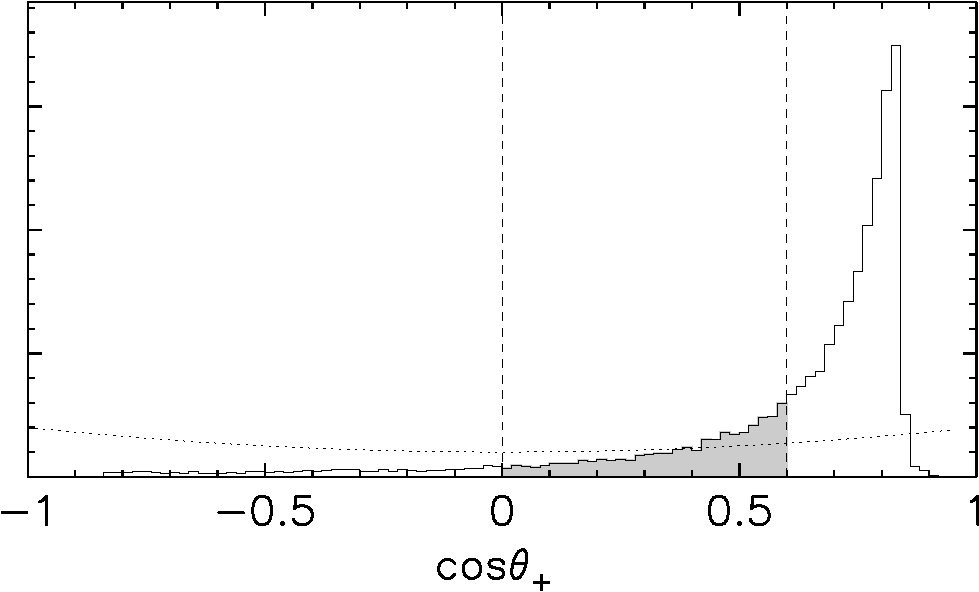
\includegraphics[width=12 cm]{/home/mccann/antithesis/plots/draw_innerbb} & &
    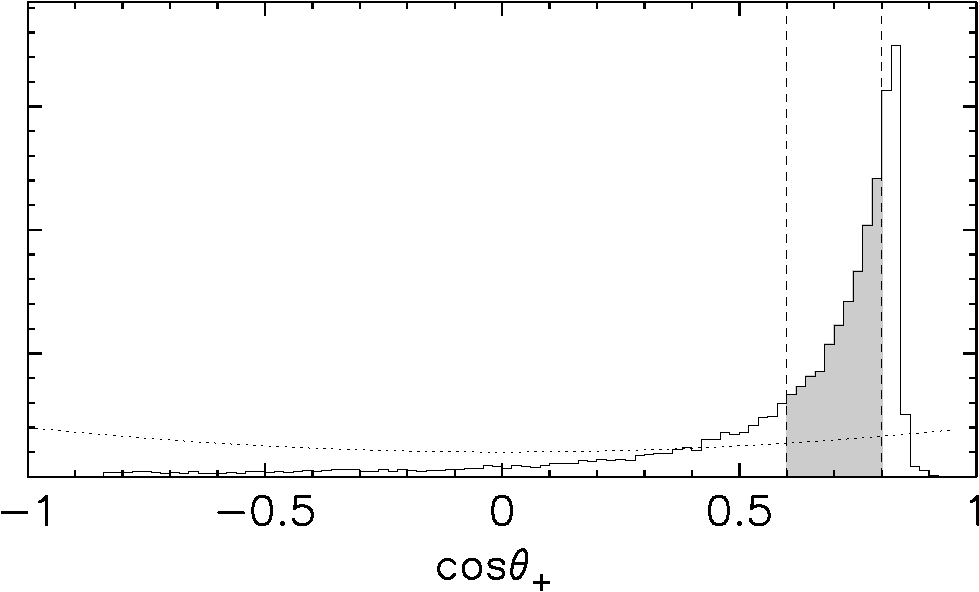
\includegraphics[width=12 cm]{/home/mccann/antithesis/plots/draw_outerbb} \\
    More contaminated by $\Upsilon \to e^+e^-$ & &
    Less contaminated by $\Upsilon \to e^+e^-$
  \end{tabular}
\end{center}

\vfill
\begin{center}
  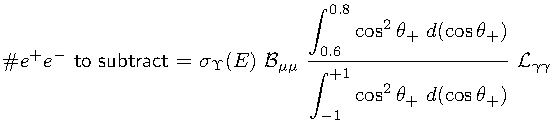
\includegraphics[width=0.75\linewidth]{equation}
\end{center}
where $\sigma_\Upsilon(E)$ is Karl's lineshape function, appropriately normalized

\vspace{-1 cm}

\end{slide}

\begin{slide}[Issue: Removing $\Upsilon \to e^+e^-$ Contamination]

$\sigma_\Upsilon(E)$ calculates Breit-Wigner $\otimes$ beam-energy spread $\otimes$ ISR tail

\vfill
with continuum (Bhabha) interference

\vfill
\begin{center}
  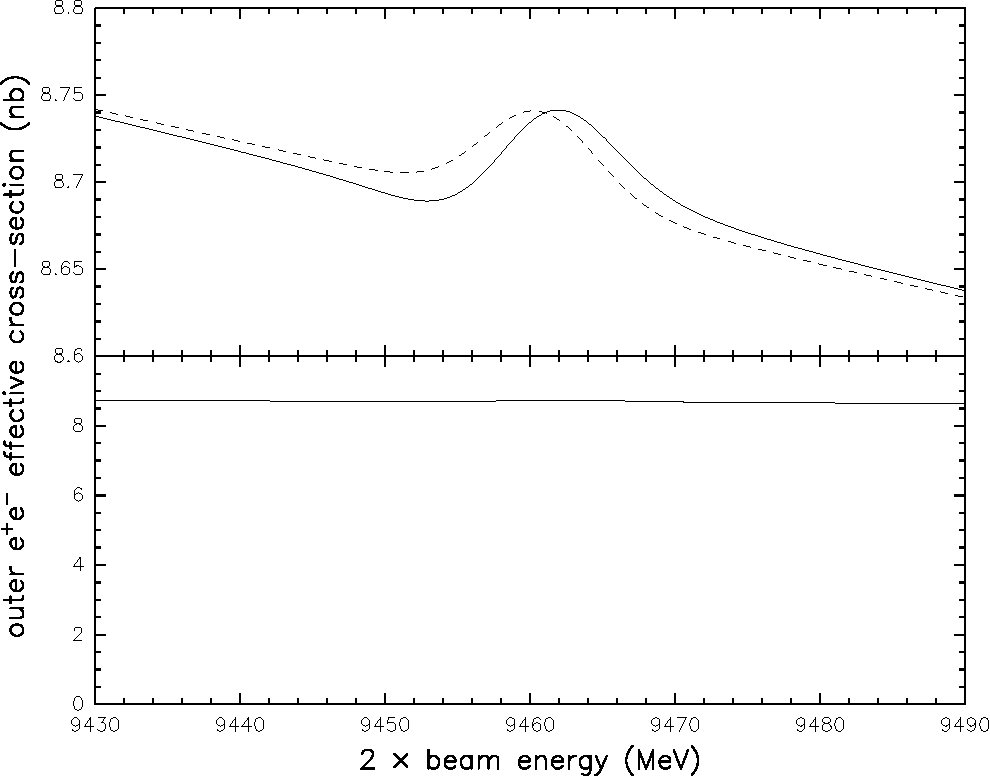
\includegraphics[width=0.65\linewidth]{/home/mccann/antithesis/plots/bbout_effective_crosssection}
\end{center}

\vfill
Solid line is $e^+e^-$ effective cross-section, dashed line is without interference

\vspace{-0.5 cm}

\end{slide}

\begin{slide}[Fit Results]

$\surd$ Including/excluding interference is a 0.02\% (0.04\%) difference for outer (inner) $e^+e^-$

\vfill
$\surd$ Outer and inner $e^+e^-$ agree with each other:

\vfill
\begin{center}
  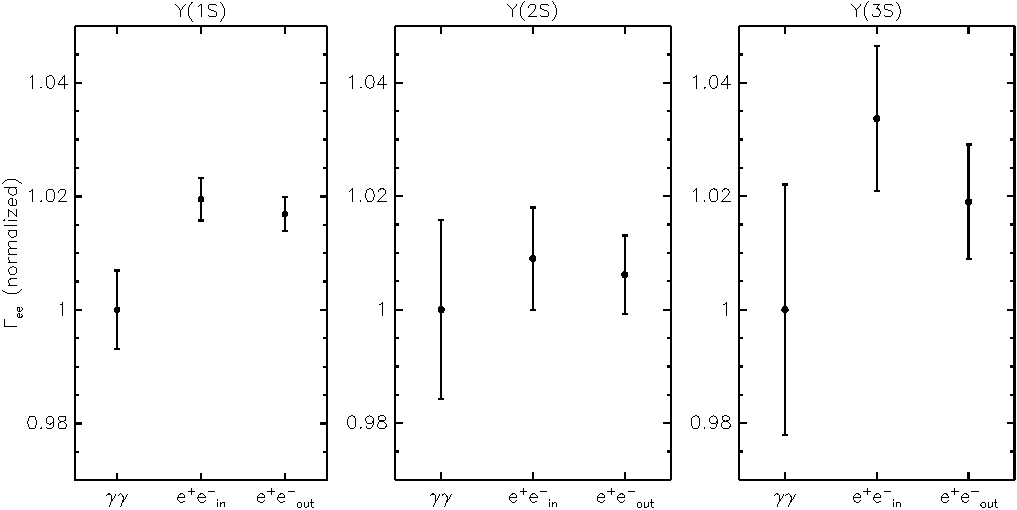
\includegraphics[width=\linewidth]{octoberfits_fixen_summaryplot}
\end{center}

\vfill
\ldots but not with $\gamma\gamma$?  I am investigating this.

\vspace{-0.5 cm}

\end{slide}

\begin{slide}

\begin{center}
  New topic: what $e^+e^-$ precision uncovered
\end{center}

\end{slide}

\begin{slide}[What $e^+e^-$ precision uncovered]

With scan data near the $\Upsilon(1S)$ peak (black = $\gamma\gamma$, {\color{red} red} = outer $e^+e^-$, grouped by week):

\vfill
\begin{center}
  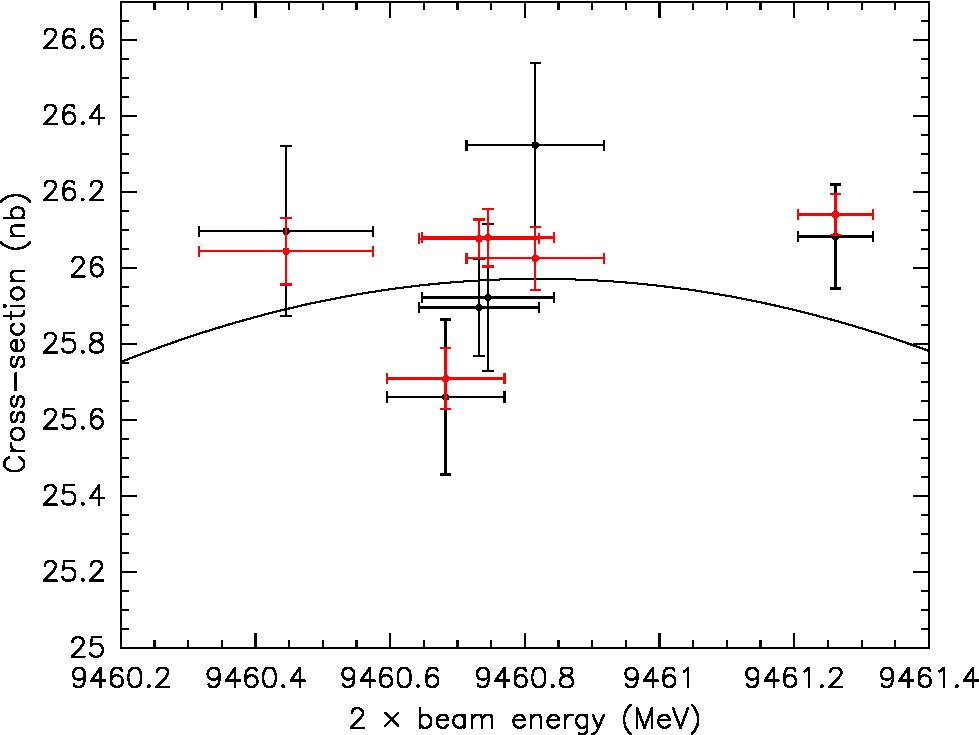
\includegraphics[width=0.8\linewidth]{/home/mccann/antithesis/plots/stability4_48hour}
\end{center}

\vfill
we see a 1.8\% excess in April 2002 (far right point)

\vspace{-1 cm}

\end{slide}

\begin{slide}[What $e^+e^-$ precision uncovered]

With {\color{red} all available CLEO-III data} with the same dates (black = $\gamma\gamma$, {\color{red} red} = outer $e^+e^-$):

\vfill
\begin{center}
  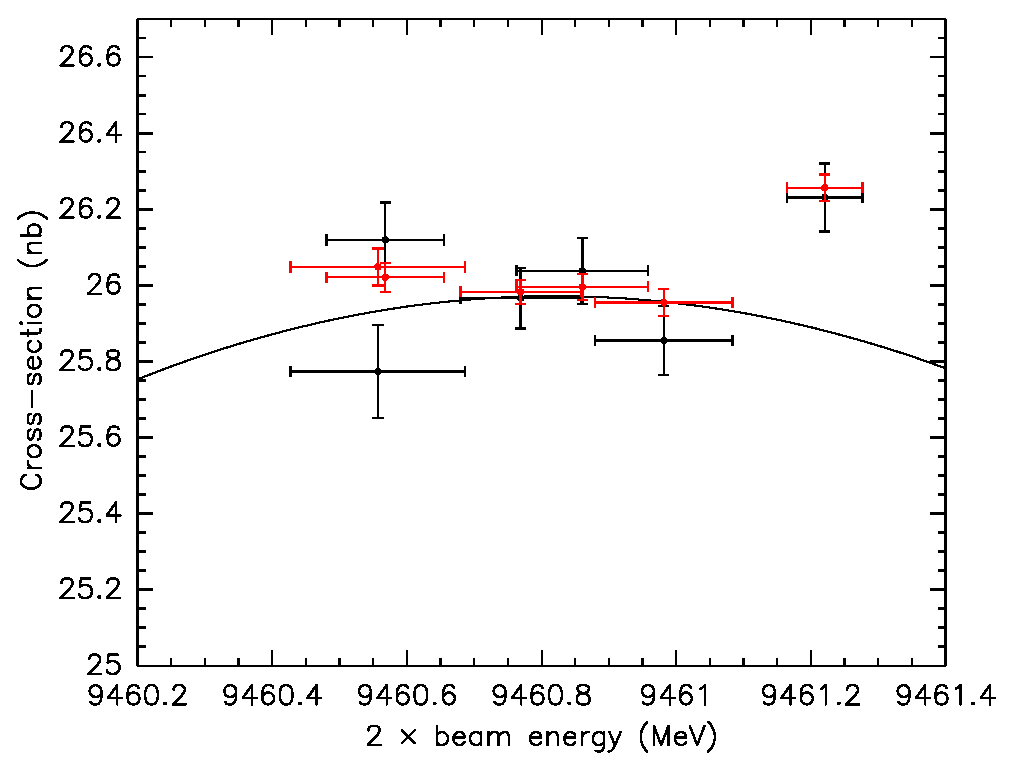
\includegraphics[width=0.8\linewidth]{/home/mccann/antithesis/plots/stability4_unlimited}
\end{center}

\vfill
we see a {\color{red} clearer} 1.8\% excess in April 2002 (far right point)

\vspace{-1 cm}

\end{slide}

\begin{slide}[What does this excess look like?]

In all distributions, the excess is distributed like $\Upsilon$
events.

\vfill
\begin{center}
  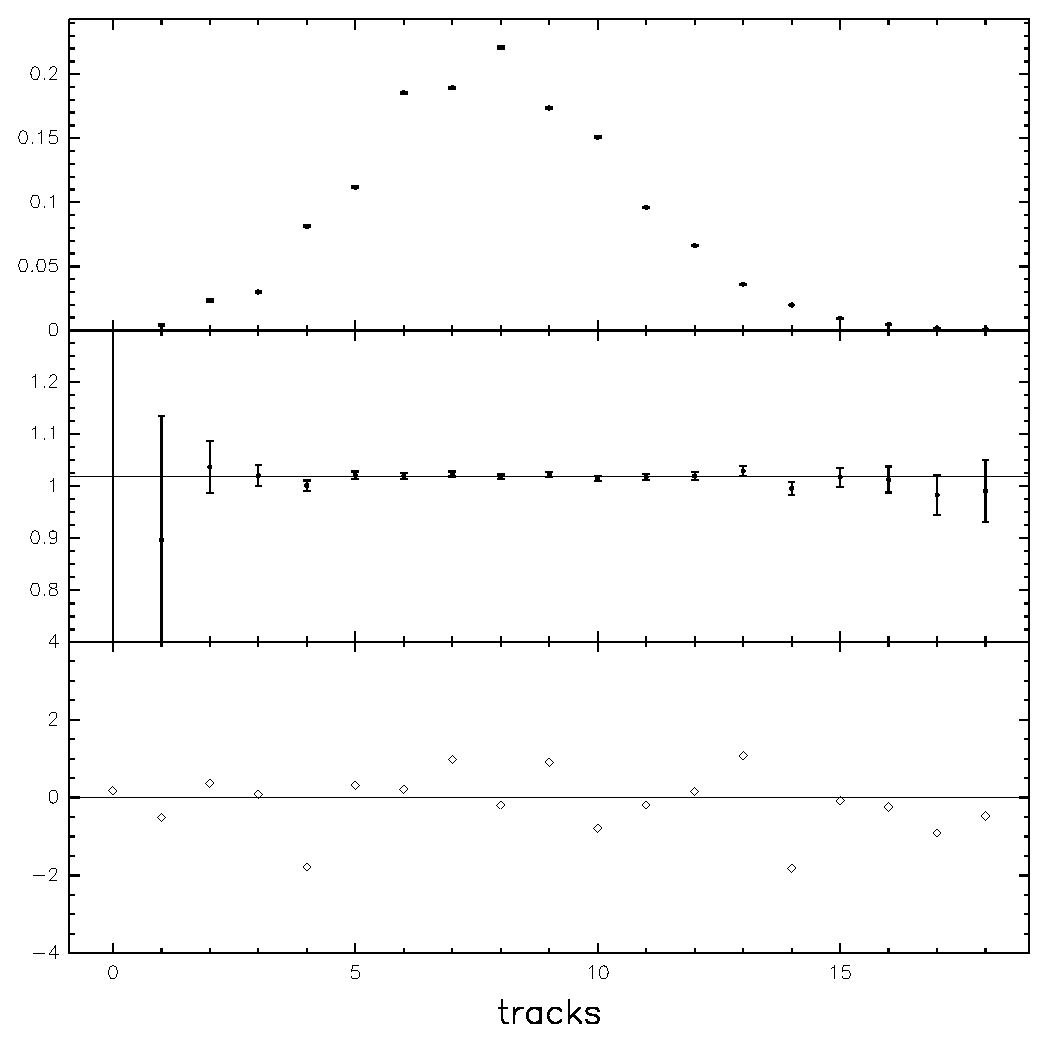
\includegraphics[width=0.55\linewidth]{/cdat/daf9/mccann/synthesis/rootstab_home/rootstab9_tracks}
\end{center}

$\rightarrow$ not an inefficiency or background

\vfill
Can $\Upsilon$ beam energy spread fluctuate on this scale?

\vspace{-1 cm}

\end{slide}

\begin{slide}[CESRV simulations]

Yes!

\vfill Simulations of an April 2002 beam orbit and a March 2002 beam
orbit reveal beam energy spread differences on the order of 1\%

\vfill Simulations with spring 2002 savesets are correlated with
measured beam energy spreads:

\vfill
\begin{center}
  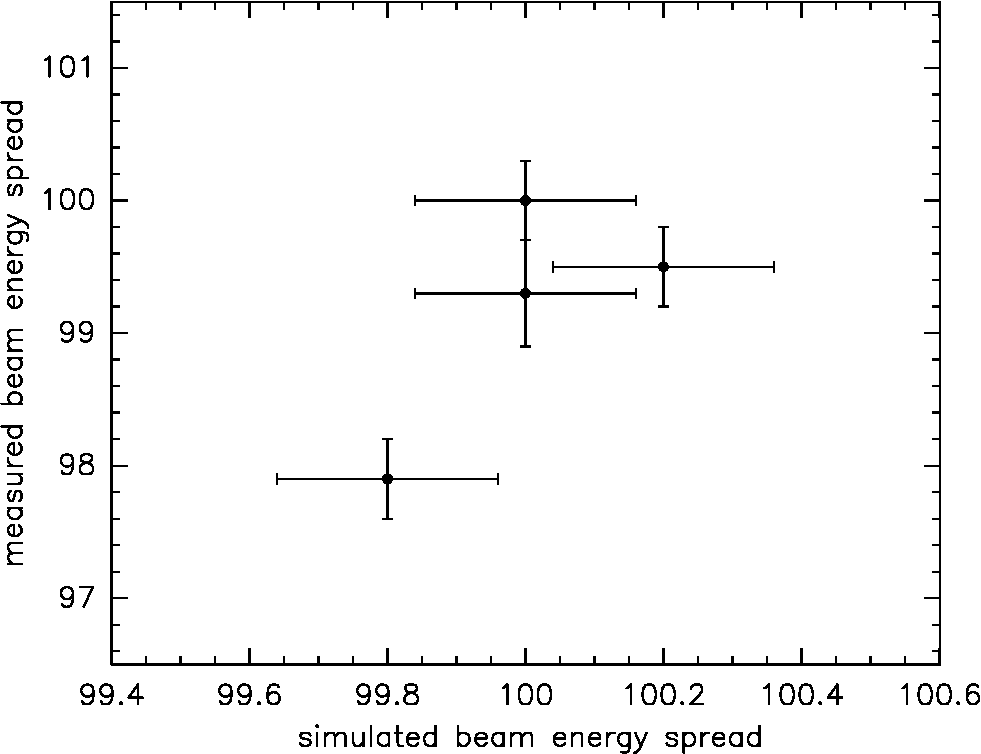
\includegraphics[width=0.5\linewidth]{/home/mccann/antithesis/plots/cesrv_correlation}
\end{center}

\vfill Surveyed CESR e-log to find breakpoints;

fits now allow piecewise constant beam energy spread

\vspace{-1 cm}

\end{slide}

\begin{slide}[Piecewise constant beam energy spread--- Fit Results]

\vfill

\begin{center}
  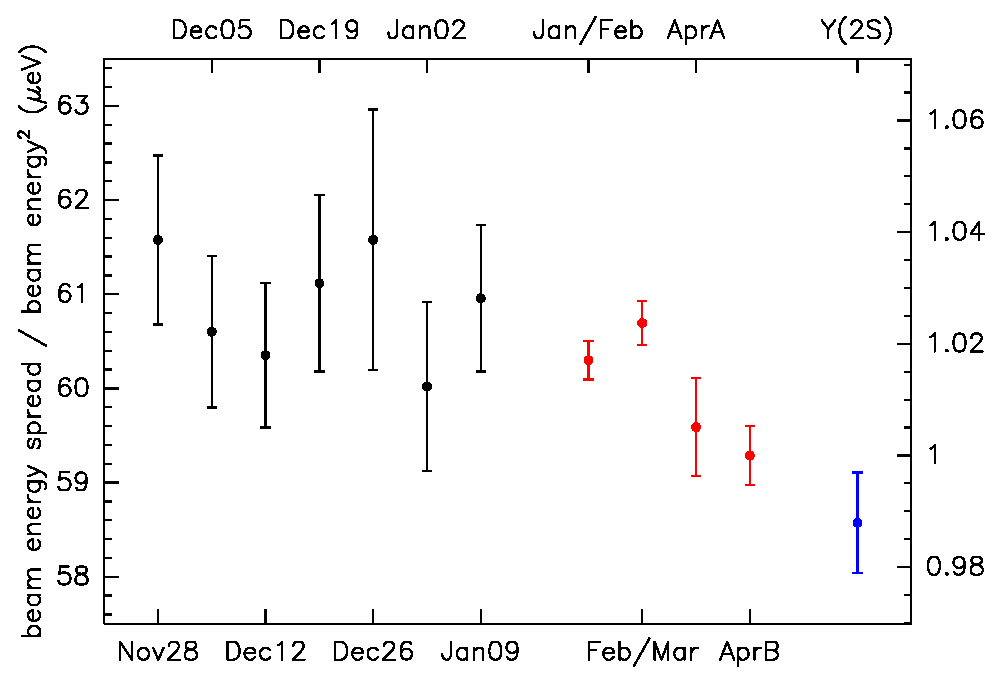
\includegraphics[width=0.9\linewidth]{piecewise_constant_beamspread}
\end{center}

\vfill
(black = $\Upsilon(3S)$, {\color{red} red} = $\Upsilon(1S)$, {\color{blue} blue} = $\Upsilon(2S)$)

\vspace{-1 cm}

\end{slide}

\begin{slide}

\begin{center}
  New topic: quality of fits
\end{center}

\end{slide}

\begin{slide}[Outer $e^+e^-$ Fit Results]

\vfill
\begin{center}
  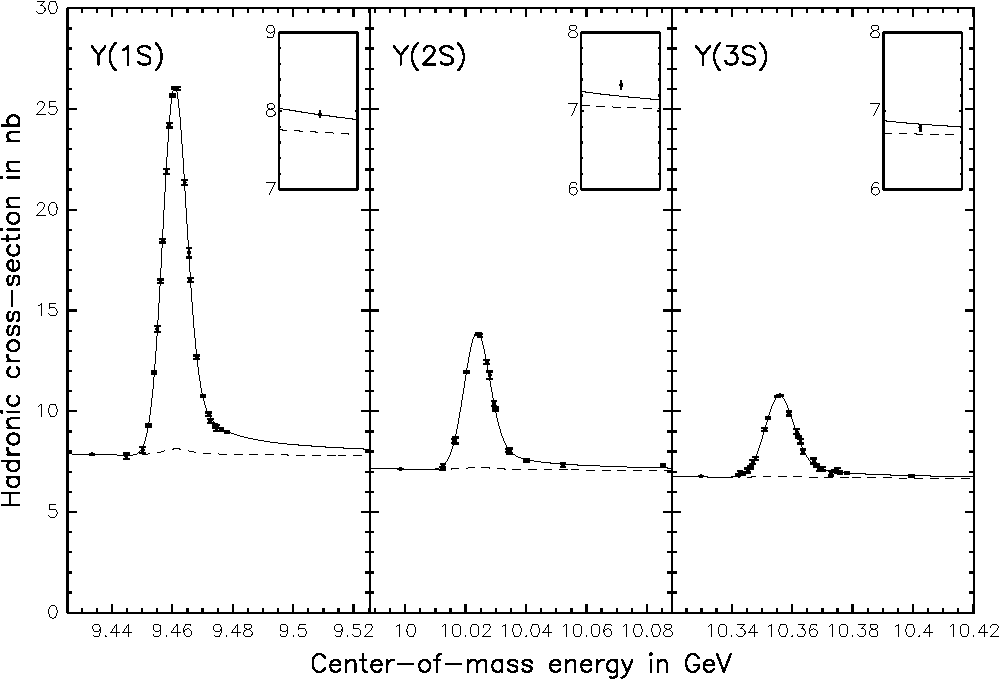
\includegraphics[width=\linewidth]{octoberfits_fixen_2_10_three_resonances_inset_squat2}
\end{center}

\vspace{-1 cm}

\end{slide}

\begin{slide}[Outer $e^+e^-$ Fit Results: $\Upsilon(1S)$ has $\chi^2$/ndf = $257.2/(210-18) = {\color{red} 1.34}$]

\vfill

\vfill
\begin{center}
  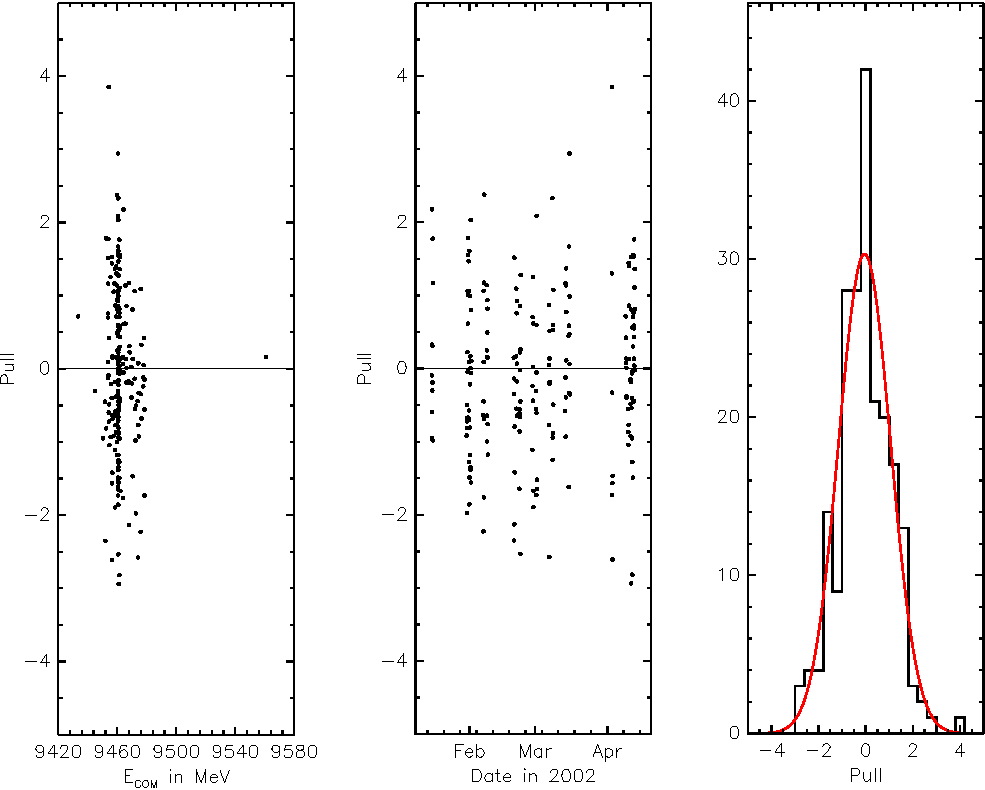
\includegraphics[width=0.8\linewidth]{octoberfits_fixen_2_10_pulls1}
\end{center}

\end{slide}

\begin{slide}[Outer $e^+e^-$ Fit Results: $\Upsilon(2S)$ has $\chi^2$/ndf = $82.0/(75-9) = {\color{red} 1.24}$]

\vfill

\vfill
\begin{center}
  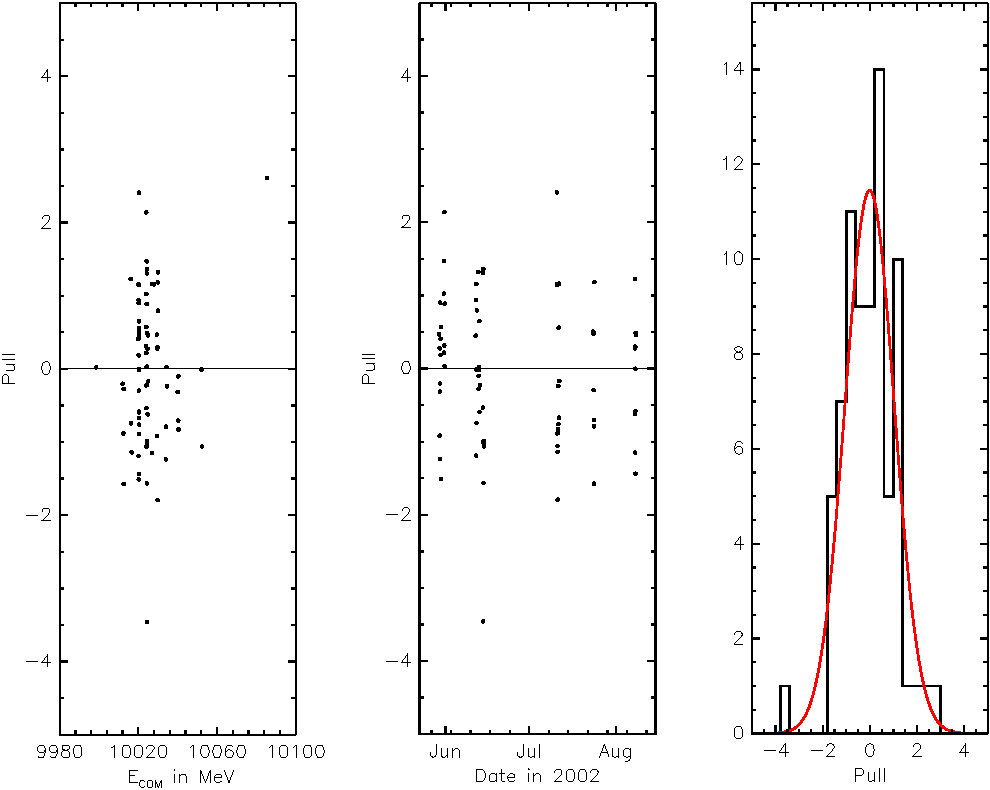
\includegraphics[width=0.8\linewidth]{octoberfits_fixen_2_10_pulls2}
\end{center}

\end{slide}

\begin{slide}[Outer $e^+e^-$ Fit Results: $\Upsilon(3S)$ has $\chi^2$/ndf = $149.93/(175-16) = {\color{red} 0.94}$]

\vfill

\vfill
\begin{center}
  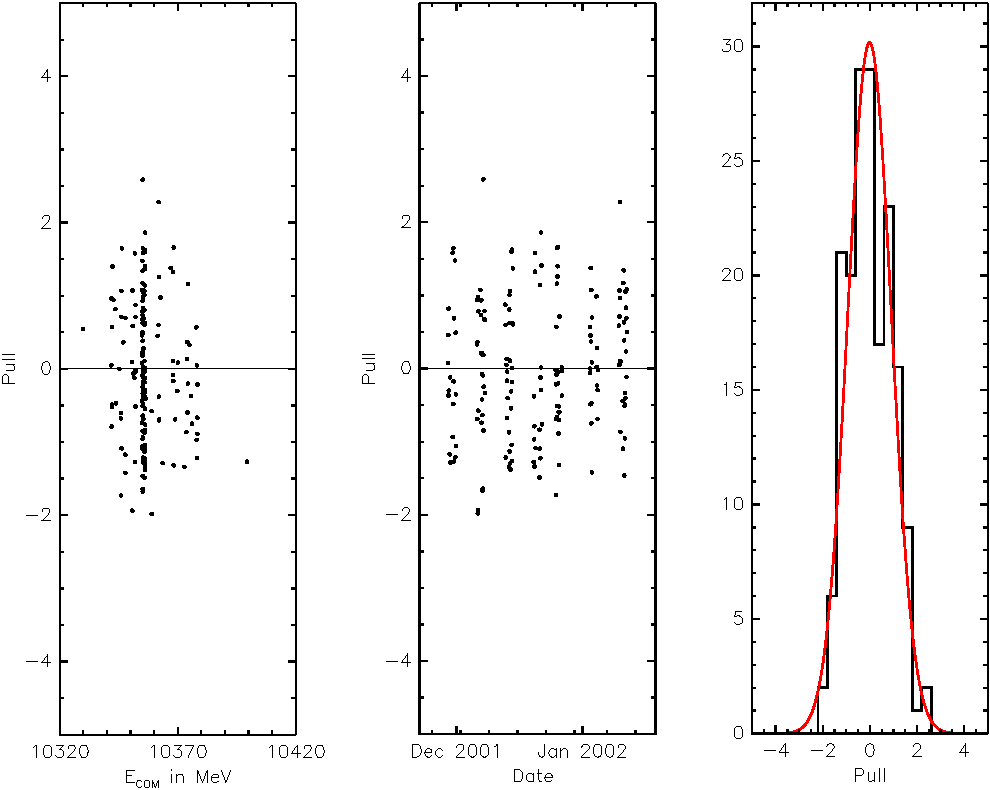
\includegraphics[width=0.8\linewidth]{octoberfits_fixen_2_10_pulls3}
\end{center}

\end{slide}

\begin{slide}[Conclusions]

\begin{itemize}\setlength{\itemsep}{0.6 cm}

  \item Subtracting $\Upsilon \to e^+e^-$ from $e^+e^-$ luminosity counts is not hard, even with interference

  \item I will use Brian and Surik's Bhabha cuts (CBX 05-17) instead of ``inner'' and ``outer''

  \item 2-$\sigma$ disagreement between $\gamma\gamma$ and $e^+e^-$ fit results?  I will check $\displaystyle \frac{\#\gamma\gamma}{\mbox{Bhabha}}$ vs.\ $E$, date

  \begin{center}
    
\includegraphics[width=0.8\linewidth]{justaline}
  \end{center}

  \item We can see one change in beam energy spread and have guarded against bias in the fit

  \begin{center}
    
\includegraphics[width=0.8\linewidth]{justaline}
  \end{center}

  \item Fit pull distributions (reduced $\chi^2$) are a little wide (1.34, 1.24, 0.94)

  \item Increase ``cross-section reproducibility'' systematic from 0.1\% to 0.4\%

  \begin{center}
    
\includegraphics[width=0.8\linewidth]{justaline}
  \end{center}

  \item Immediately after PANIC, we start to write the PRL

  \item Paper vote in December!

\end{itemize}

\end{slide}





\end{document}
